% Chapter 10: Comprehensive Review - Complete Time Series Analysis
% Applying all methods to real data
% Bachelor program, Bucharest University of Economic Studies

\documentclass[9pt, aspectratio=169, t]{beamer}

% Ensure content fits on slides
\setbeamersize{text margin left=8mm, text margin right=8mm}

%=============================================================================
% THEME AND STYLE CONFIGURATION
%=============================================================================
\usetheme{Madrid}
\usecolortheme{seahorse}

% IDA-Inspired Color Palette
\definecolor{MainBlue}{RGB}{26, 58, 110}
\definecolor{AccentBlue}{RGB}{42, 82, 140}
\definecolor{IDAred}{RGB}{220, 53, 69}
\definecolor{DarkGray}{RGB}{51, 51, 51}
\definecolor{MediumGray}{RGB}{128, 128, 128}
\definecolor{LightGray}{RGB}{248, 248, 248}
\definecolor{VeryLightGray}{RGB}{235, 235, 235}
\definecolor{Crimson}{RGB}{220, 53, 69}
\definecolor{Forest}{RGB}{46, 125, 50}
\definecolor{Amber}{RGB}{181, 133, 63}
\definecolor{Orange}{RGB}{230, 126, 34}

\setbeamercolor{palette primary}{bg=MainBlue, fg=white}
\setbeamercolor{palette secondary}{bg=MainBlue!85, fg=white}
\setbeamercolor{palette tertiary}{bg=MainBlue!70, fg=white}
\setbeamercolor{structure}{fg=MainBlue}
\setbeamercolor{title}{fg=MainBlue}
\setbeamercolor{frametitle}{fg=MainBlue, bg=white}
\setbeamercolor{block title}{bg=MainBlue, fg=white}
\setbeamercolor{block body}{bg=VeryLightGray, fg=DarkGray}
\setbeamercolor{block title alerted}{bg=Crimson, fg=white}
\setbeamercolor{block body alerted}{bg=Crimson!8, fg=DarkGray}
\setbeamercolor{block title example}{bg=Forest, fg=white}
\setbeamercolor{block body example}{bg=Forest!8, fg=DarkGray}
\setbeamercolor{item}{fg=MainBlue}

\setbeamertemplate{navigation symbols}{}

\setbeamertemplate{footline}{
    \leavevmode%
    \hbox{%
        \begin{beamercolorbox}[wd=.333333\paperwidth,ht=2.5ex,dp=1ex,center]{author in head/foot}%
            \usebeamerfont{author in head/foot}\insertshortauthor
        \end{beamercolorbox}%
        \begin{beamercolorbox}[wd=.333333\paperwidth,ht=2.5ex,dp=1ex,center]{title in head/foot}%
            \usebeamerfont{title in head/foot}\insertshorttitle
        \end{beamercolorbox}%
        \begin{beamercolorbox}[wd=.333333\paperwidth,ht=2.5ex,dp=1ex,right]{date in head/foot}%
            \usebeamerfont{date in head/foot}\insertshortdate{}\hspace*{2em}
            \insertframenumber{} / \inserttotalframenumber\hspace*{2ex}
        \end{beamercolorbox}}%
    \vskip0pt%
}

%=============================================================================
% PACKAGES
%=============================================================================
\usepackage[utf8]{inputenc}
\usepackage[T1]{fontenc}
\usepackage{amsmath, amssymb, amsthm}
\usepackage{mathtools}
\usepackage{bm}
\usepackage{tikz}
\usetikzlibrary{arrows.meta, positioning, shapes, calc}
\usepackage{booktabs}
\usepackage{multirow}
\usepackage{array}
\usepackage{graphicx}
\usepackage{hyperref}
\hypersetup{colorlinks=false, pdfborder={0 0 0}}
\graphicspath{{../logos/}{../charts/}}

%=============================================================================
% THEOREM ENVIRONMENTS
%=============================================================================
\theoremstyle{definition}
\setbeamertemplate{theorems}[numbered]
\newtheorem{defn}{Definition}
\newtheorem{thm}{Theorem}
\newtheorem{prop}{Proposition}

%=============================================================================
% CUSTOM COMMANDS
%=============================================================================
\newcommand{\E}{\mathbb{E}}
\newcommand{\Var}{\text{Var}}
\newcommand{\Cov}{\text{Cov}}
\newcommand{\Corr}{\text{Corr}}
\newcommand{\R}{\mathbb{R}}

%=============================================================================
% TITLE INFORMATION
%=============================================================================
\title[Chapter 10: Comprehensive Review]{Chapter 10: Comprehensive Review}
\subtitle{Complete Time Series Analysis with Real Data}
\author{Daniel Traian Pele}
\institute[ASE]{
    Bucharest University of Economic Studies\\
    Faculty of Cybernetics, Statistics, and Economic Informatics\\
    \texttt{daniel.pele@csie.ase.ro}
}
\date{Academic Year 2025-2026}

\begin{document}

%=============================================================================
% TITLE SLIDE
%=============================================================================
\begin{frame}
    \titlepage
    \begin{center}
        \includegraphics[width=0.15\textwidth]{logo_csie.png}
        \hspace{1cm}
        \includegraphics[width=0.15\textwidth]{logo_ase.png}
    \end{center}
\end{frame}

%=============================================================================
% TABLE OF CONTENTS
%=============================================================================
\begin{frame}{Outline}
    \tableofcontents
\end{frame}

%=============================================================================
% SECTION 1: INTRODUCTION
%=============================================================================
\section{The Complete Analysis Workflow}

\begin{frame}{Course Overview: Methods Covered}
    \begin{columns}[T]
        \begin{column}{0.48\textwidth}
            \textbf{Classical Methods}
            \begin{itemize}
                \item \textcolor{MainBlue}{Ch 1:} Time Series Fundamentals
                \item \textcolor{MainBlue}{Ch 2:} ARMA Models
                \item \textcolor{MainBlue}{Ch 3:} ARIMA Models
                \item \textcolor{MainBlue}{Ch 4:} SARIMA Models
                \item \textcolor{MainBlue}{Ch 5:} GARCH Models
            \end{itemize}
        \end{column}
        \begin{column}{0.48\textwidth}
            \textbf{Advanced Methods}
            \begin{itemize}
                \item \textcolor{Forest}{Ch 6:} VAR \& Granger Causality
                \item \textcolor{Forest}{Ch 7:} Cointegration \& VECM
                \item \textcolor{Forest}{Ch 8:} Modern Extensions
                \item \textcolor{Forest}{Ch 9:} Prophet \& TBATS
            \end{itemize}
            \vspace{0.5em}
            \textbf{Today: Apply ALL to Real Data!}
        \end{column}
    \end{columns}
\end{frame}

\begin{frame}{The Complete Analysis Workflow}
    \begin{center}
        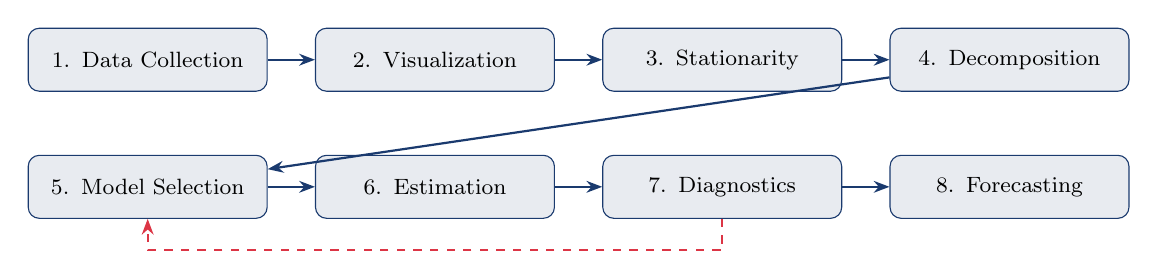
\begin{tikzpicture}[
            node distance=0.6cm,
            box/.style={rectangle, rounded corners, draw=MainBlue, fill=MainBlue!10,
                        text width=2.8cm, minimum height=0.8cm, align=center, font=\footnotesize},
            arrow/.style={-{Stealth[length=2mm]}, thick, MainBlue}
        ]
            % Row 1
            \node[box] (data) {1. Data Collection};
            \node[box, right=of data] (viz) {2. Visualization};
            \node[box, right=of viz] (stat) {3. Stationarity};
            \node[box, right=of stat] (decomp) {4. Decomposition};

            % Row 2
            \node[box, below=0.8cm of data] (model) {5. Model Selection};
            \node[box, right=of model] (est) {6. Estimation};
            \node[box, right=of est] (diag) {7. Diagnostics};
            \node[box, right=of diag] (forecast) {8. Forecasting};

            % Arrows
            \draw[arrow] (data) -- (viz);
            \draw[arrow] (viz) -- (stat);
            \draw[arrow] (stat) -- (decomp);
            \draw[arrow] (decomp) -- (model);
            \draw[arrow] (model) -- (est);
            \draw[arrow] (est) -- (diag);
            \draw[arrow] (diag) -- (forecast);

            % Feedback loop
            \draw[arrow, dashed, IDAred] (diag.south) -- ++(0,-0.4) -| (model.south);
        \end{tikzpicture}
    \end{center}

    \vspace{0.3cm}
    \begin{alertblock}{Key Principle}
        Model diagnostics may require returning to model selection (iterative process)
    \end{alertblock}
\end{frame}

\begin{frame}{Real Datasets for This Chapter}
    \begin{columns}[T]
        \begin{column}{0.32\textwidth}
            \begin{block}{S\&P 500 Returns}
                \begin{itemize}
                    \item Daily financial data
                    \item 2019-2024
                    \item Volatility clustering
                    \item ARIMA + GARCH
                \end{itemize}
            \end{block}
        \end{column}
        \begin{column}{0.32\textwidth}
            \begin{block}{Air Passengers}
                \begin{itemize}
                    \item Monthly 1949-1960
                    \item Classic dataset
                    \item Trend + seasonality
                    \item SARIMA vs Prophet
                \end{itemize}
            \end{block}
        \end{column}
        \begin{column}{0.32\textwidth}
            \begin{block}{US Retail Sales}
                \begin{itemize}
                    \item Monthly 2018-2023
                    \item FRED economic data
                    \item COVID-19 impact
                    \item Structural breaks
                \end{itemize}
            \end{block}
        \end{column}
    \end{columns}
\end{frame}

%=============================================================================
% SECTION 2: CASE STUDY 1 - FINANCIAL DATA
%=============================================================================
\section{Case Study 1: S\&P 500 Financial Analysis}

\begin{frame}{S\&P 500: Data Overview}
    \begin{center}
        \includegraphics[width=0.95\textwidth, height=0.70\textheight, keepaspectratio]{ch10_sp500_overview.pdf}
    \end{center}

    \begin{itemize}
        \item \textbf{Data:} S\&P 500 daily closing prices and returns (2019-2024)
        \item \textbf{Key events:} COVID-19 crash (March 2020), recovery, 2022 bear market
    \end{itemize}
\end{frame}

\begin{frame}{Step 1: Stationarity Testing}
    \begin{columns}[T]
        \begin{column}{0.55\textwidth}
            \textbf{Augmented Dickey-Fuller Test}
            \begin{itemize}
                \item $H_0$: Unit root (non-stationary)
                \item $H_1$: Stationary
            \end{itemize}

            \vspace{0.5em}
            \textbf{Results on S\&P 500:}
            \begin{table}[h]
                \footnotesize
                \begin{tabular}{lcc}
                    \toprule
                    Series & ADF Statistic & p-value \\
                    \midrule
                    Prices & $-1.23$ & 0.66 \\
                    Returns & $-35.2$ & $<0.001$ \\
                    \bottomrule
                \end{tabular}
            \end{table}

            \vspace{0.5em}
            $\Rightarrow$ Prices: non-stationary \\
            $\Rightarrow$ Returns: stationary
        \end{column}
        \begin{column}{0.43\textwidth}
            \begin{exampleblock}{KPSS Test (Confirmation)}
                \begin{itemize}
                    \item $H_0$: Stationary
                    \item $H_1$: Unit root
                \end{itemize}

                \vspace{0.3em}
                Prices: KPSS = 4.21** \\
                Returns: KPSS = 0.08

                \vspace{0.3em}
                \textcolor{Forest}{Both tests confirm: use returns!}
            \end{exampleblock}
        \end{column}
    \end{columns}
\end{frame}

\begin{frame}{Step 2: ACF/PACF Analysis of Returns}
    \begin{center}
        \includegraphics[width=0.95\textwidth, height=0.65\textheight, keepaspectratio]{ch10_sp500_acf_pacf.pdf}
    \end{center}

    \begin{itemize}
        \item \textbf{Returns:} Near white noise (weak autocorrelation)
        \item \textbf{Squared returns:} Strong persistence $\Rightarrow$ volatility clustering
        \item \textbf{Implication:} Need GARCH for volatility modeling
    \end{itemize}
\end{frame}

\begin{frame}{Step 3: ARIMA Model for Returns}
    \textbf{Model Selection using AIC/BIC:}

    \begin{columns}[T]
        \begin{column}{0.48\textwidth}
            \begin{table}[h]
                \footnotesize
                \begin{tabular}{lcc}
                    \toprule
                    Model & AIC & BIC \\
                    \midrule
                    ARIMA(0,0,0) & -8234 & -8228 \\
                    ARIMA(1,0,0) & -8236 & -8224 \\
                    ARIMA(0,0,1) & -8235 & -8223 \\
                    \textbf{ARIMA(1,0,1)} & \textbf{-8238} & \textbf{-8220} \\
                    \bottomrule
                \end{tabular}
            \end{table}

            \vspace{0.3em}
            Best model: ARIMA(1,0,1) or simple mean model
        \end{column}
        \begin{column}{0.48\textwidth}
            \begin{alertblock}{Key Insight}
                Stock returns are nearly unpredictable (efficient market hypothesis). The real story is in the \textbf{volatility}, not the mean!
            \end{alertblock}
        \end{column}
    \end{columns}
\end{frame}

\begin{frame}{Step 4: GARCH Model for Volatility}
    \begin{center}
        \includegraphics[width=0.95\textwidth, height=0.60\textheight, keepaspectratio]{ch10_sp500_garch.pdf}
    \end{center}

    \textbf{GARCH(1,1) Model:}
    \[
        \sigma_t^2 = \omega + \alpha \varepsilon_{t-1}^2 + \beta \sigma_{t-1}^2
    \]

    \begin{itemize}
        \item High $\alpha + \beta \approx 0.98$ indicates strong volatility persistence
        \item COVID-19 period shows massive volatility spike
    \end{itemize}
\end{frame}

\begin{frame}{Financial Data: Summary of Approach}
    \begin{center}
        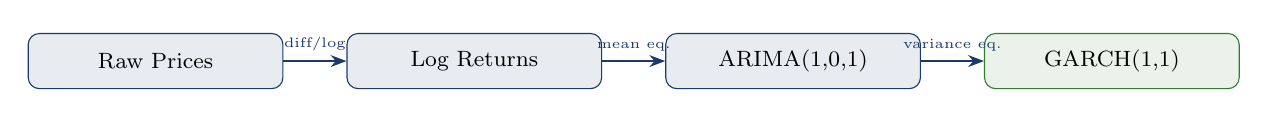
\begin{tikzpicture}[
            node distance=0.4cm,
            box/.style={rectangle, rounded corners, draw=MainBlue, fill=MainBlue!10,
                        text width=3cm, minimum height=0.7cm, align=center, font=\footnotesize},
            result/.style={rectangle, rounded corners, draw=Forest, fill=Forest!10,
                          text width=3cm, minimum height=0.7cm, align=center, font=\footnotesize},
            arrow/.style={-{Stealth[length=2mm]}, thick, MainBlue}
        ]
            \node[box] (prices) {Raw Prices};
            \node[box, right=0.8cm of prices] (returns) {Log Returns};
            \node[box, right=0.8cm of returns] (arima) {ARIMA(1,0,1)};
            \node[result, right=0.8cm of arima] (garch) {GARCH(1,1)};

            \draw[arrow] (prices) -- node[above, font=\tiny] {diff/log} (returns);
            \draw[arrow] (returns) -- node[above, font=\tiny] {mean eq.} (arima);
            \draw[arrow] (arima) -- node[above, font=\tiny] {variance eq.} (garch);
        \end{tikzpicture}
    \end{center}

    \vspace{0.5em}
    \begin{columns}[T]
        \begin{column}{0.48\textwidth}
            \textbf{Key Findings:}
            \begin{itemize}
                \item Returns are nearly unpredictable
                \item Volatility clusters significantly
                \item GARCH captures risk dynamics
            \end{itemize}
        \end{column}
        \begin{column}{0.48\textwidth}
            \textbf{Practical Use:}
            \begin{itemize}
                \item Risk management (VaR)
                \item Option pricing
                \item Portfolio optimization
            \end{itemize}
        \end{column}
    \end{columns}
\end{frame}

%=============================================================================
% SECTION 3: CASE STUDY 2 - SEASONAL DATA
%=============================================================================
\section{Case Study 2: Air Passengers with Seasonality}

\begin{frame}{Air Passengers: The Classic Dataset}
    \begin{center}
        \includegraphics[width=0.95\textwidth, height=0.65\textheight, keepaspectratio]{ch10_airpassengers_overview.pdf}
    \end{center}

    \begin{itemize}
        \item \textbf{Data:} Monthly airline passengers (thousands), 1949-1960
        \item \textbf{Characteristics:} Upward trend + yearly seasonality + multiplicative pattern
    \end{itemize}
\end{frame}

\begin{frame}{Step 1: Decomposition Analysis}
    \begin{center}
        \includegraphics[width=0.95\textwidth, height=0.65\textheight, keepaspectratio]{ch10_airpassengers_decomposition.pdf}
    \end{center}

    \begin{itemize}
        \item \textbf{Trend:} Strong upward growth (aviation industry expansion)
        \item \textbf{Seasonal:} Peak in summer (July-August), trough in winter
        \item \textbf{Multiplicative:} Seasonal amplitude grows with level
    \end{itemize}
\end{frame}

\begin{frame}{Step 2: Making Data Stationary}
    \textbf{Transformations Applied:}
    \begin{enumerate}
        \item Log transformation (stabilize variance)
        \item First difference (remove trend)
        \item Seasonal difference (remove seasonality)
    \end{enumerate}

    \vspace{0.5em}
    \begin{columns}[T]
        \begin{column}{0.48\textwidth}
            \begin{table}[h]
                \footnotesize
                \begin{tabular}{lc}
                    \toprule
                    Series & ADF p-value \\
                    \midrule
                    Original & 0.99 \\
                    Log & 0.42 \\
                    Log + Diff & 0.07 \\
                    Log + Diff + SDiff & $<0.01$ \\
                    \bottomrule
                \end{tabular}
            \end{table}
        \end{column}
        \begin{column}{0.48\textwidth}
            \textbf{SARIMA notation:}
            \[
                \text{SARIMA}(p,d,q)(P,D,Q)_s
            \]

            For Air Passengers:
            \begin{itemize}
                \item $d=1$ (first difference)
                \item $D=1$ (seasonal difference)
                \item $s=12$ (monthly seasonality)
            \end{itemize}
        \end{column}
    \end{columns}
\end{frame}

\begin{frame}{Step 3: SARIMA Model Fitting}
    \begin{columns}[T]
        \begin{column}{0.48\textwidth}
            \textbf{Model Selection:}
            \begin{table}[h]
                \footnotesize
                \begin{tabular}{lc}
                    \toprule
                    Model & AIC \\
                    \midrule
                    $(1,1,1)(1,1,1)_{12}$ & 1020.3 \\
                    $(0,1,1)(0,1,1)_{12}$ & 1018.7 \\
                    \textbf{$(2,1,1)(0,1,1)_{12}$} & \textbf{1017.1} \\
                    $(1,1,0)(1,1,0)_{12}$ & 1025.4 \\
                    \bottomrule
                \end{tabular}
            \end{table}

            \vspace{0.3em}
            Best: SARIMA$(2,1,1)(0,1,1)_{12}$
        \end{column}
        \begin{column}{0.48\textwidth}
            \textbf{Model Equation:}
            \[
                (1-\phi_1 B - \phi_2 B^2)(1-B)(1-B^{12})y_t
            \]
            \[
                = (1+\theta_1 B)(1+\Theta_1 B^{12})\varepsilon_t
            \]

            \vspace{0.5em}
            \textbf{Diagnostics:}
            \begin{itemize}
                \item Ljung-Box: p = 0.42
                \item Residuals: white noise
            \end{itemize}
        \end{column}
    \end{columns}
\end{frame}

\begin{frame}{Step 4: Prophet as Alternative}
    \begin{center}
        \includegraphics[width=0.95\textwidth, height=0.60\textheight, keepaspectratio]{ch10_airpassengers_prophet.pdf}
    \end{center}

    \textbf{Prophet Model:}
    \[
        y(t) = g(t) + s(t) + h(t) + \varepsilon_t
    \]

    \begin{itemize}
        \item Trend $g(t)$: Piecewise linear with changepoints
        \item Seasonality $s(t)$: Fourier series (multiplicative mode)
    \end{itemize}
\end{frame}

\begin{frame}{SARIMA vs Prophet: Comparison}
    \begin{center}
        \includegraphics[width=0.95\textwidth, height=0.55\textheight, keepaspectratio]{ch10_airpassengers_comparison.pdf}
    \end{center}

    \begin{table}[h]
        \footnotesize
        \centering
        \begin{tabular}{lccc}
            \toprule
            Model & RMSE & MAE & MAPE (\%) \\
            \midrule
            SARIMA$(2,1,1)(0,1,1)_{12}$ & 18.2 & 14.5 & 3.1 \\
            Prophet (multiplicative) & 21.4 & 17.2 & 3.7 \\
            TBATS & 19.8 & 15.9 & 3.4 \\
            \bottomrule
        \end{tabular}
    \end{table}

    \textbf{Conclusion:} SARIMA slightly better for this classic, well-behaved dataset
\end{frame}

%=============================================================================
% SECTION 4: CASE STUDY 3 - ECONOMIC DATA WITH STRUCTURAL BREAK
%=============================================================================
\section{Case Study 3: US Retail Sales with Structural Break}

\begin{frame}{US Retail Sales: COVID-19 Impact}
    \begin{center}
        \includegraphics[width=0.95\textwidth, height=0.65\textheight, keepaspectratio]{ch10_retail_overview.pdf}
    \end{center}

    \begin{itemize}
        \item \textbf{Data:} US Retail Sales, monthly, 2018-2023 (FRED)
        \item \textbf{Challenge:} Major structural break in March-April 2020
    \end{itemize}
\end{frame}

\begin{frame}{Handling Structural Breaks}
    \begin{columns}[T]
        \begin{column}{0.48\textwidth}
            \textbf{Option 1: Truncate Data}
            \begin{itemize}
                \item Use only post-COVID data
                \item Pro: Clean, no breaks
                \item Con: Lose historical info
            \end{itemize}

            \vspace{0.5em}
            \textbf{Option 2: Dummy Variables}
            \begin{itemize}
                \item Add COVID indicator
                \item Pro: Uses all data
                \item Con: Complex in ARIMA
            \end{itemize}
        \end{column}
        \begin{column}{0.48\textwidth}
            \textbf{Option 3: Prophet with Changepoints}
            \begin{itemize}
                \item Automatic detection
                \item Pro: Handles breaks naturally
                \item Con: May overfit
            \end{itemize}

            \vspace{0.5em}
            \begin{exampleblock}{Recommendation}
                For COVID-impacted data, Prophet's changepoint detection or post-COVID truncation often works best.
            \end{exampleblock}
        \end{column}
    \end{columns}
\end{frame}

\begin{frame}{Prophet for Retail Sales}
    \begin{center}
        \includegraphics[width=0.95\textwidth, height=0.60\textheight, keepaspectratio]{ch10_retail_prophet.pdf}
    \end{center}

    \textbf{Prophet Configuration:}
    \begin{itemize}
        \item \texttt{changepoint\_prior\_scale = 0.1} (flexible for COVID)
        \item \texttt{seasonality\_mode = 'multiplicative'}
        \item Automatic changepoint detection captures the break
    \end{itemize}
\end{frame}

\begin{frame}{Model Comparison on Retail Sales}
    \begin{table}[h]
        \centering
        \begin{tabular}{lccc}
            \toprule
            Model & RMSE (\$B) & MAE (\$B) & MAPE (\%) \\
            \midrule
            SARIMA (full data) & 42.1 & 35.8 & 6.2 \\
            SARIMA (post-COVID) & 18.3 & 14.7 & 2.4 \\
            \textbf{Prophet (with breaks)} & \textbf{15.2} & \textbf{12.1} & \textbf{2.0} \\
            TBATS & 19.4 & 15.8 & 2.6 \\
            \bottomrule
        \end{tabular}
    \end{table}

    \vspace{0.5em}
    \begin{alertblock}{Key Lesson}
        When data has structural breaks, traditional ARIMA struggles. Prophet's flexibility with changepoints makes it better suited for such scenarios.
    \end{alertblock}
\end{frame}

%=============================================================================
% SECTION 5: MODEL SELECTION GUIDE
%=============================================================================
\section{Model Selection: A Practical Guide}

\begin{frame}{Decision Framework}
    \begin{center}
        \includegraphics[width=0.90\textwidth, height=0.70\textheight, keepaspectratio]{ch10_model_selection_flowchart.pdf}
    \end{center}
\end{frame}

\begin{frame}{Model Selection Summary}
    \begin{table}[h]
        \footnotesize
        \centering
        \begin{tabular}{p{2.5cm}p{3.5cm}p{3.5cm}p{3cm}}
            \toprule
            \textbf{Data Type} & \textbf{Characteristics} & \textbf{Recommended Model} & \textbf{Alternatives} \\
            \midrule
            Financial returns & No trend, volatility clustering & ARIMA-GARCH & EGARCH, GJR \\
            \addlinespace
            Single seasonality & Trend + one seasonal period & SARIMA & ETS, Prophet \\
            \addlinespace
            Multiple seasonality & Daily + weekly + annual & Prophet, TBATS & Dynamic regression \\
            \addlinespace
            Structural breaks & COVID, regime changes & Prophet & Piecewise regression \\
            \addlinespace
            Multiple series & Interdependencies & VAR, VECM & Factor models \\
            \bottomrule
        \end{tabular}
    \end{table}
\end{frame}

\begin{frame}{Forecast Evaluation Metrics}
    \begin{columns}[T]
        \begin{column}{0.48\textwidth}
            \textbf{Point Forecast Metrics:}

            \vspace{0.3em}
            \textbf{RMSE} (Root Mean Square Error):
            \[
                \sqrt{\frac{1}{n}\sum_{i=1}^{n}(y_i - \hat{y}_i)^2}
            \]

            \textbf{MAE} (Mean Absolute Error):
            \[
                \frac{1}{n}\sum_{i=1}^{n}|y_i - \hat{y}_i|
            \]

            \textbf{MAPE} (Mean Absolute \% Error):
            \[
                \frac{100}{n}\sum_{i=1}^{n}\left|\frac{y_i - \hat{y}_i}{y_i}\right|
            \]
        \end{column}
        \begin{column}{0.48\textwidth}
            \textbf{When to Use Each:}
            \begin{itemize}
                \item \textbf{RMSE}: Penalizes large errors more
                \item \textbf{MAE}: Robust to outliers
                \item \textbf{MAPE}: Scale-independent
            \end{itemize}

            \vspace{0.5em}
            \begin{alertblock}{Cross-Validation}
                Always use time series CV:
                \begin{itemize}
                    \item Rolling window
                    \item Expanding window
                    \item Never shuffle!
                \end{itemize}
            \end{alertblock}
        \end{column}
    \end{columns}
\end{frame}

%=============================================================================
% SECTION 6: SUMMARY
%=============================================================================
\section{Summary and Key Takeaways}

\begin{frame}{Course Summary: Complete Toolkit}
    \begin{columns}[T]
        \begin{column}{0.48\textwidth}
            \textbf{Understanding the Data}
            \begin{itemize}
                \item Visualization first!
                \item Test for stationarity (ADF, KPSS)
                \item Identify seasonality patterns
                \item Check for structural breaks
            \end{itemize}

            \vspace{0.5em}
            \textbf{Classical Models}
            \begin{itemize}
                \item ARIMA: Non-seasonal data
                \item SARIMA: Single seasonality
                \item GARCH: Volatility modeling
            \end{itemize}
        \end{column}
        \begin{column}{0.48\textwidth}
            \textbf{Modern Approaches}
            \begin{itemize}
                \item Prophet: Interpretable, handles breaks
                \item TBATS: Multiple seasonalities
                \item VAR/VECM: Multiple time series
            \end{itemize}

            \vspace{0.5em}
            \textbf{Best Practices}
            \begin{itemize}
                \item Always check diagnostics
                \item Use cross-validation
                \item Compare multiple models
                \item Domain knowledge matters!
            \end{itemize}
        \end{column}
    \end{columns}
\end{frame}

\begin{frame}{Final Recommendations}
    \begin{enumerate}
        \item \textbf{Start Simple}: Begin with visualization and basic statistics
        \item \textbf{Test Assumptions}: Stationarity, normality, independence
        \item \textbf{Iterate}: Model $\rightarrow$ Diagnose $\rightarrow$ Improve
        \item \textbf{Compare}: Never rely on a single model
        \item \textbf{Validate}: Out-of-sample testing is essential
        \item \textbf{Communicate}: Clear visualizations and interpretations
    \end{enumerate}

    \vspace{0.5em}
    \begin{exampleblock}{Remember}
        ``All models are wrong, but some are useful.'' --- George Box

        \vspace{0.3em}
        The goal is not perfect prediction, but useful insights and reasonable forecasts.
    \end{exampleblock}
\end{frame}

\begin{frame}{Thank You!}
    \begin{center}
        \Large
        \textbf{Questions?}

        \vspace{1cm}

        \normalsize
        Course Materials: \texttt{github.com/danpele/Time-Series-Analysis}

        \vspace{0.5cm}

        Contact: \texttt{daniel.pele@csie.ase.ro}

        \vspace{1cm}

        \includegraphics[width=0.12\textwidth]{logo_csie.png}
        \hspace{1cm}
        \includegraphics[width=0.12\textwidth]{logo_ase.png}
    \end{center}
\end{frame}

\end{document}
